\subsection{Javascript}

\citeonline{javascript_diego_leonard}, afirmam que o Javascript foi criado e lançado pela Netscape em 1995, em conjunto com o navegador de internet Netscape Navigator 2.0. A partir deste lançamento, as páginas \textit{web} passaram a ganhar vida com a possibilidade de implementar um mínimo de dinamicidade devido ao modo como a linguagem acessa e manipula os componentes do navegador. Contudo, ela pode ser utilizada em difentes dispositivos como \textit{smartphones, smart tv}, entre outros, não limitando-se apenas à navegadores de internet.

O Javascript é uma linguagem de programação para \textit{web}. A maioria dos sites usam esta linguagem, inclusive todos os navegadores mais modernos, vídeo games, \textit{tablets}, \textit{smart phones}, \textit{smart tvs} possuem interpretadores de \textit{Javascript}, o que a fez tornar, a linguagem de programação mais ambígua da história \cite{flanagan_javascript_definitive_guide}.

Segundo \citeonline{javascript_diego_leonard}, as semelhanças entre o Javascript e o Java se limitam apenas ao nome. A primeira linguagem não deriva da segunda, apesar de ambas compartilharem alguns conceitos e detalhes. O Javascript por ser uma linguagem interpretada, é mais flexível que o Java que, por sua vez, é uma linguagem compilada.

De acordo com \citeonline{flanagan_javascript_definitive_guide}, o Javascript possui 6 versões, sendo elas: 1.0, 1.1, 1.2, 1.3, 1.4 e a atual versão 1.5.

Para \citeonline{javascript_diego_leonard}, há duas maneiras de incluir e executar o Javascript em documentos HTML. A primeira é incluir o código Javascript entre as \textit{tags} \texttt{script} como mostra a fígura 13. 

\begin{figure}[h!]
	\centerline{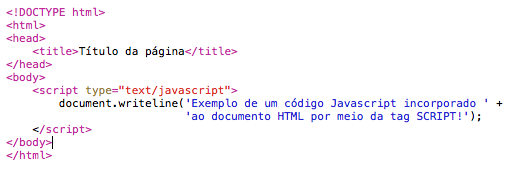
\includegraphics[scale=0.8]{./imagens/javascript_code.png}}
	\caption[Exemplo de inclusão do código em Javascript incorporado ao HTML]
	{Exemplo de inclusão do código em Javascript incorporado ao HTML. \textbf{Fonte:} Elaborado pelos autores.}
	\label{fig:exemplo1}
\end{figure}

A segunda forma é incluir um arquivo externo com extensão \texttt{.js} através da mesma \textit{tag} \texttt{script}, veja um exemplo de inclusão de um arquivo contendo códigos em Javascript no documento HTML na figura 14.

\begin{figure}[h!]
	\centerline{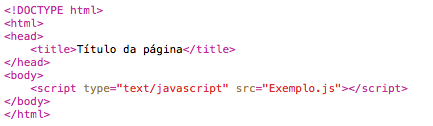
\includegraphics[scale=0.8]{./imagens/javascript_include.png}}
	\caption[Exemplo de inclusão do código Javascript de um arquivo externo]
	{Exemplo de inclusão do código Javascript de um arquivo externo. \textbf{Fonte:} Elaborado pelos autores.}
	\label{fig:exemplo1}
\end{figure}

Para \citeonline{flanagan_javascript_definitive_guide}, as três tecnologias (HTML, CSS e Javascript) devem ser usadas em conjunto, uma vez que, cada uma delas possui seu papel específico, sendo eles: o HTML usado para especificar o conteúdo da página \textit{web}, o CSS para especificar como os componentes serão apresentados na página \textit{web} e o Javascript para especificar o comportamento da página \textit{web}.

Pelos motivos acima mencionados, somado ao fato que o Javascript permite ao desenvolvedor criar páginas \textit{web} mais dinâmicas e flexíveis, atendendo perfeitamente os requisitos deste projeto. Esta tecnologia será utilizada para auxiliar a criação das páginas \textit{web} deste \textit{software}.